\section{DRL Commands}
\subsection{Select}


\begin{prettyBox}{Select}{myblue}
To display the contents of one or more tables at once, we use the \textcolor{blue}{SELECT} command. We can choose
specific columns and tables to display, we can give aliases to tables and columns . When selecting from multiple tables of different size
, a Cartesian product occurs, meaning each row from one table is paired with each row from the other.
\end{prettyBox}

\subsubsection*{\underline{Syntax}}

\lstinputlisting{SQL/syntax/DRL/select.sql}

\subsection{Where}

\begin{prettyBox}{Where Clause}{myblue}
The \textcolor{blue}{WHERE} clause is used to filter rows in a table when displaying data with the
\textcolor{blue}{SELECT} command. Only rows that meet the specified condition(s) are shown in the result.
\end{prettyBox}

\subsubsection*{\underline{Syntax}}

\lstinputlisting{SQL/syntax/DRL/where.sql}

\subsection{Aggregation Functions}
 \begin{prettyBox}{Aggregation Functions}{myblue}
   Aggregation functions perform calculations on a set of values and return a single result. They are commonly used in conjunction with the \textcolor{blue}{GROUP BY} clause to summarize data.
   \begin{itemize}
    \item \textbf{Avg(column$_{i}$)} : Calculates the average (mean) of numeric values in a specified column.
    \item \textbf{Min(column$_{i}$)} : Returns the smallest (minimum) value in a specified column.
    \item \textbf{Max(column$_{i}$)} : Returns the largest (maximum) value in a specified column.
    \item \textbf{Count()} : Counts the number of non-null entries in a specified column (or all rows if * is used).
      \begin{itemize}
        \item  \textbf{count(*)} : Counts All rows
        \item  \textbf{count(column$_{i}$)} : counts number of rows where column$_{i}$ is not null
        \item  \textbf{count(distinct column$_{i}$)} : counts number of rows where column$_{i}$ is not null without repetition
    \end{itemize}
    \item \textbf{Sum(column$_{i}$)} : Adds up all values in a specified numeric column.
   \end{itemize} 
\end{prettyBox}

\vspace{0.25cm}

\begin{prettyBox}{Note}{red}
\begin{itemize}
    \item We can do arithmethical operations inside parameters of some aggregation functions like avg,max,min,sum 
    \item We can use nested aggregation function in some cases 
\end{itemize}
\end{prettyBox}

\vspace{0.5cm}
\subsection{Group By} 
\begin{prettyBox}{Group By}{myblue}
To group rows that have the same value in a specified column, we use the \textcolor{blue}{GROUP BY} command.
We can group by multiple columns; the order is important because it will first group by the first column. If there
are rows that have the same value in the first column but differ in the second column, those rows will appear in
separate groups in the output. This allows us to apply aggregate functions to summarize data for each group.
\end{prettyBox}

\vspace{0.25cm}
\subsubsection*{\underline{Syntax}}

\lstinputlisting{SQL/syntax/DRL/groupby.sql}


\subsection{Having}
\begin{prettyBox}{Having Clause}{myblue}

    Similar to \textcolor{blue}{WHERE}, which filters rows based on conditions, 
\textcolor{blue}{HAVING} is used to filter groups of data rather than individual rows. Unlike
\textcolor{blue}{WHERE}, which applies conditions before grouping, \textcolor{blue}{HAVING} is
applied after the \textcolor{blue}{GROUP BY} clause. This allows you to filter aggregated results.
\end{prettyBox}


\vspace{0.25cm}
\subsubsection*{\underline{Syntax}}

\lstinputlisting{SQL/syntax/DRL/having.sql}


\vspace{0.5cm}
\subsection{Order By}

\begin{prettyBox}{Order By}{myblue}
We can sort the results of a query in either ascending or descending order using \textcolor{blue}{ORDER BY}. 
This can be applied to one or multiple columns. The order of the columns specified is important; the database
first sorts by the first column, and if there are rows with identical values in that column, it then sorts those
rows by the next column, and so on. This allows for a prioritized sorting strategy.
\end{prettyBox}

\vspace{0.25cm}
\subsubsection*{\underline{Syntax}}

\lstinputlisting{SQL/syntax/DRL/orderby.sql}

\vspace{0.5cm}
\subsection{Joins}
\begin{prettyBox}{Joins}{myblue}
joins allow you to combine rows from two or more tables based on related columns (referenced key)
\end{prettyBox}

\vspace{0.25cm}
\subsubsection{Inner Joins}
\begin{prettyBox}{Inner Joins}{myblue}
An Inner Join returns only the common rows between tables
\begin{center}
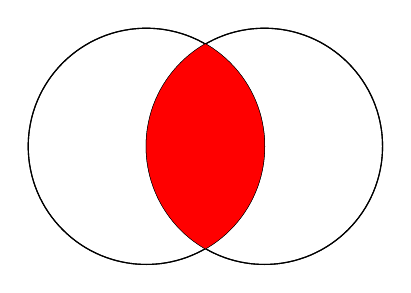
\begin{tikzpicture}
    \draw (-0.5,0) circle (1.5cm);
    \draw[black] (-0.5,0) circle (1.5cm);
    
    \draw (1,0) circle (1.5cm);
    \draw[black] (1,0) circle (1.5cm);
   \begin{scope}
        \clip (-0.5,0) circle (1.5cm);  
        \fill[red] (1,0) circle (1.5cm);  
    \end{scope} 
\end{tikzpicture}
\end{center}
\end{prettyBox}

\vspace{0.25cm}
\subsubsection{Left Join}

\begin{prettyBox}{Left Join}{myblue}
A Left Join returns all rows from the left table and the matched rows from the right table. If there’s no match,
NULL values are returned for columns from the right table.

\begin{center}
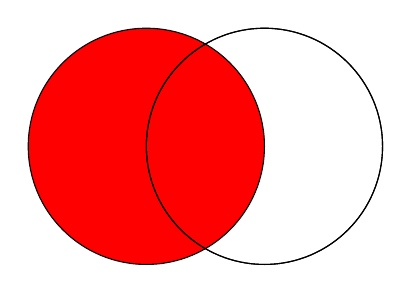
\begin{tikzpicture}
    \fill[red] (-0.5,0) circle (1.5cm);
    \draw[black] (-0.5,0) circle (1.5cm);

    \draw (1,0) circle (1.5cm);
    \draw[black] (1,0) circle (1.5cm);
\end{tikzpicture}
\end{center}
\end{prettyBox}

\vspace{0.25cm}
\subsubsection{Right Join}
\begin{prettyBox}{Right Join}{myblue}
A Right Join returns all rows from the right table and the matched rows from the left table. If there’s no match,
NULL values are returned for columns from the left table.
\begin{center}
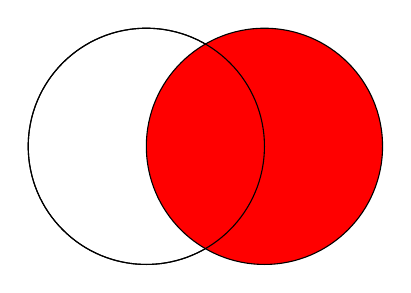
\begin{tikzpicture}
    \draw (-0.5,0) circle (1.5cm);

    \fill[red] (1,0) circle (1.5cm);

    \draw[black] (1,0) circle (1.5cm);
    \draw[black] (-0.5,0) circle (1.5cm);
\end{tikzpicture}
\end{center}
\end{prettyBox}

\vspace{0.25cm}
\subsubsection{Full Join}

\begin{prettyBox}{Full Join}{myblue}
A Full Join returns all rows when there is a match in either left or right table. If there is no match,
NULL values are returned for unmatched columns.
\begin{center}
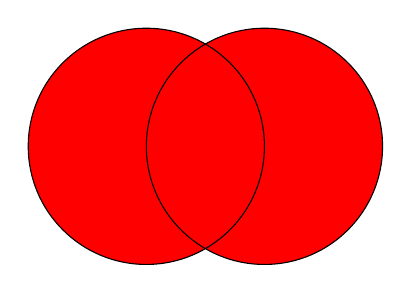
\begin{tikzpicture}
    \fill[red] (-0.5,0) circle (1.5cm);

    \fill[red] (1,0) circle (1.5cm);
    \draw[black] (1,0) circle (1.5cm);

    \draw[black] (-0.5,0) circle (1.5cm);
\end{tikzpicture}
\end{center}
\end{prettyBox}

\vspace{0.25cm}
\subsubsection*{ \textbf{Syntax}}

\lstinputlisting{SQL/syntax/DRL/joins.sql}

\vspace{0.25cm}
\begin{prettyBox}{Note}{red}
We can have different types of joins in one select query
\end{prettyBox}

\vspace{0.5cm}
\subsection{Operators}
\begin{prettyBox}{Operators}{myblue}
Operators are symbols that specify operations to be performed on operands. They can be categorized as follows:
\end{prettyBox}

\vspace{0.25cm}
\subsubsection{Logical Operators}
\begin{prettyBox}{Logical}{myblue}
Used to combine conditions.
          \begin{itemize} 
              \item Logical And : AND 
              \item Logical Or : OR 
              \item Logical Not : NOT 
              \end{itemize} 
\end{prettyBox}

\vspace{0.25cm}
\subsubsection{Comparison Operators}
\begin{prettyBox}{Comparison}{myblue}
Used to compare values.
    \begin{itemize}
             \item Equal : = 
             \item Not Equal : != 
             \item Greater : \textgreater
             \item Greater Or Equal : \textgreater= 
             \item Less : \textless
             \item Less Or Equal : \textless= 
             \item Between : BETWEEN value$_{1}$ AND value$_{2}$
             \item In : IN (set of values)
             \end{itemize} 
\end{prettyBox}

\vspace{0.25cm}
\subsubsection{Arithmetic Operators}
\begin{prettyBox}{Arithmetic}{myblue}
Used for mathematical calculations.
    \begin{itemize} 
           \item Multiplication : *
           \item Division : / 
           \item Sum : + 
           \item Subtraction : -
           \end{itemize}
\end{prettyBox}

\subsection{Query Execution Order}

\vspace{0.5cm}
\begin{center}
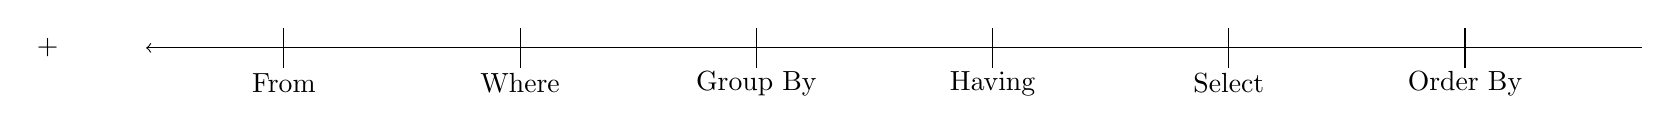
\begin{tikzpicture}
    \draw[<-] (1,0) -- (20,0);
    
    \draw (2.75,-0.25) -- (2.75,0.25);
    \node at (2.75,-0.45) {From};
    
    \draw (5.75,-0.25) -- (5.75,0.25);
    \node at (5.75,-0.45) {Where};
    
    \draw (8.75,-0.25) -- (8.75,0.25);
    \node at (8.75,-0.45) {Group By};

    \draw (11.75,-0.25) -- (11.75,0.25);
    \node at (11.75,-0.45) {Having};

    \draw (14.75,-0.25) -- (14.75,0.25);
    \node at (14.75,-0.45) {Select};

    \draw (17.75,-0.25) -- (17.75,0.25);
    \node at (17.75,-0.45) {Order By};

    \node at (-0.25,0) {+};



\end{tikzpicture}
\end{center}

